% !TEX root = thesis.tex
\graphicspath{{./figures/}}

%%%%%%%%%%%%%%%%%%%%%%%%
\chapter{Implementation}
%%%%%%%%%%%%%%%%%%%%%%%%

To explore the two approaches, they were implemented in Python. Python is versatile, simple, and offers a large collection of helpful libraries like NetworkX, a library for working with graphs. \TODO{cite: https://networkx.org/documentation/stable/index.html}

Furthermore, each implementation was deliberately structured into two distinct phases: set-up and solving, to enable meaningful runtime benchmarking. The algorithms take python dictionaries, called "dicts", as inputs, which map a key to a value. \TODO{cite https://docs.python.org/3/tutorial/datastructures.html} The delegation graph is represented in a "dict of dicts" format, where every key in the dict is a node, and the value is another dict, with the node's neighbours as keys, and a weight as value. The input is an "inverse" delegation graph in so far as that the inner dicts are the incoming delegations, as opposed containing outgoing edges. \Cref{fig:inverse_dict_example} shows an example of this. Since the implementations require inputs in different formats, conversions from a dict-of-dicts to the appropriate format are necessary. However, including the set-up time in benchmarks may be misleading, as this time is not spent on actually resolving delegations. That said, in practice, the set-up time can be a relevant factor—depending on the use case and data format—when choosing between different approaches or implementations. The set-up procedures required for each implementation are described in more detail in the sections below.

\begin{figure}[t]
    \centering
    \begin{subfigure}[t]{0.45\textwidth}
        \centering
        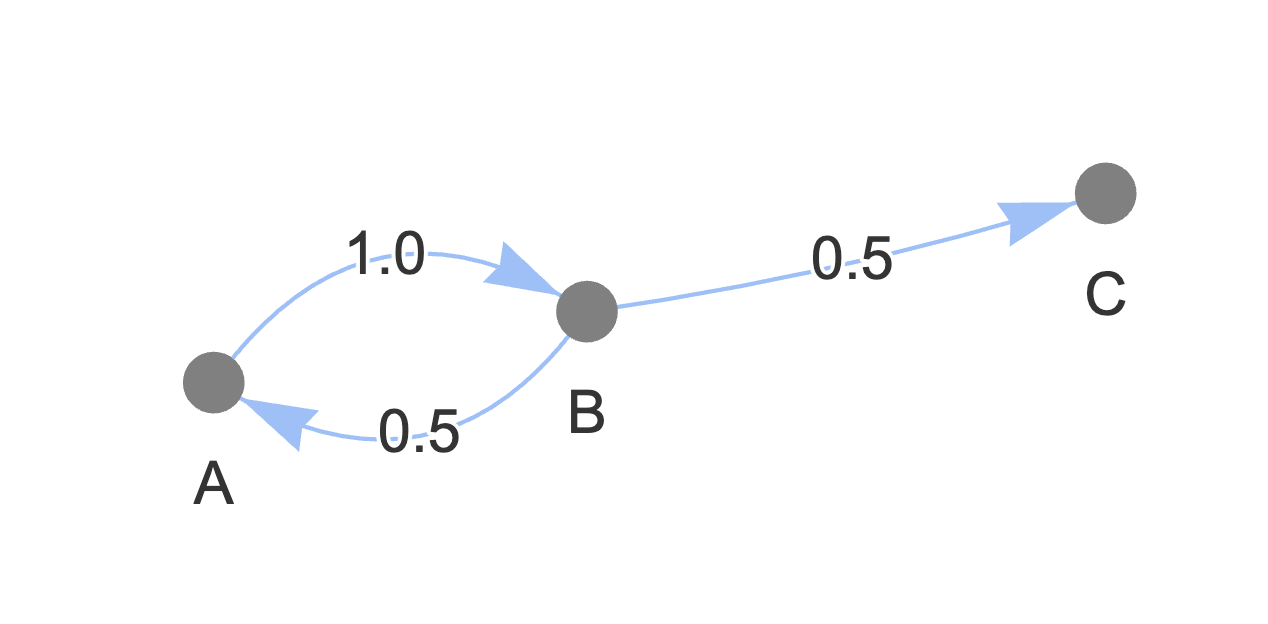
\includegraphics[width=\textwidth]{small_cycle_graph}
        \caption{Delegation graph}
    \end{subfigure}
    \hfill
    \begin{subfigure}[t]{0.45\textwidth}
        \centering
        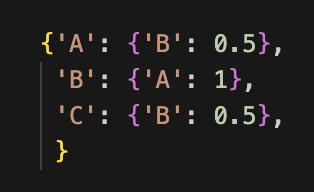
\includegraphics[width=\textwidth]{small_cycle_graph_inverse_dict}
        \caption{Inverse dict representation}
    \end{subfigure}
    \caption{Delegation graphs and its inverse dict representation}
    \label{fig:inverse_dict_example}
\end{figure}



\section{Iterative Approach}

The implementation of the iterative approach is based closely on the pseudocode of \cref{alg:iterative_with_cutoff}. After being initialised to 1, the algorithm iteratively takes a snapshot of power values in the graph, and then distributes them according to the delegations, until the change in power each round falls below a cutoff value. 

The code takes the dict-of-dicts representation of the delegation graph, a list of nodes, as well as a cutoff value as parameters, and returns the dict mapping nodes to their power values. The list of nodes must contain all the nodes in the graph since otherwise the code will not know about any nodes which have no incoming delegations. As discussed in \cref{sec:iterative_approach}, the cutoff value is necessary to ensure that the algorithm terminates in finite steps.

\section{System of Linear Equations Approach}

We try and compare two different approaches for resolving delegations using the systems of linear equations approach.

\subsection{Linear Programming Solver Implementation (LP Implementation)}

For this approach, we use the Python library PuLP, which provides an interface to Linear Programming (LP) solvers. \TODO{cite https://coin-or.github.io/pulp/} To resolve the delegation graphs, we use the "Coin-or branch and cut" (CBC) solver, since it is free and open-source. Given the academic context and the moderate size of our delegation graphs, CBC provides a practical balance between performance and accessibility. Moreover, since our model essentially solves a system of linear equations with a unique correct solution, the choice of solver has little influence on the outcome itself — even if CBC is not the most optimised solver for this class of problems. While commercial solvers may offer faster runtimes, CBC is sufficient for our use case and ensures reproducibility without licensing constraints.

The algorithm first sets up the linear program, setting up an equation $p'_v = \sum_{(u, v, w) \in E} 1 + wp'_u$ for each node $v \in V$. This is then solved by the CBC solver, with the primal tolerance set to $5*10^{-3}$ to level the playing field compared to the iterative algorithm, which does not have perfect accuracy either. A tolerance of $5 * 10^{-3}$ assures that $\lvert p'_v -\sum_{(u, v, w) \in E} 1 + wp'_u \rvert \le 5*10^{-3}$, so the solutions will be correct when rounded to the second decimal place. Finally, the algorithm cleans the $p_v'$ values, setting any delegators power to 0. 

%\TODO{\text{cite: https://jump.dev/JuMP.jl/stable/tutorials/getting_started/tolerances/#:~:text=The\%20primal\%20feasibility\%20tolerance\%20controls,model)\%20is\_solved\_and\_feasible(model)\%20false}}

\subsection{Linear System Solver Implementation (LS Implementation)}

Secondly, we use a a dedicated linear system solver. We try SciPy's \texttt{scipy.sparse.linalg.spsolve} solver, which is optimized for sparse matrices.\TODO{insert missing citation} A sparse solver is better equipped to resolve delegations if we assume that realistically each delegator only delegates to a few delegates. Since each $wp_v$ term in the system of linear equations can be mapped to one unique edge $(u, v, p) \in E$, the matrix corresponding to the system of linear equations likely has relatively few non zero entries compared to its size. In other words:

\[
\text{For a small } n \in \mathbb{N} \text{, and a large |V|}, D \subset V: n \cdot |D| < |V| \cdot |V|
\]

 \TODO{This explanation is ugly, but idk if its worth spending a lot more time on...}
 
 The implementation makes use of SciPy's Compressed Sparse Column (CSC) arrays, which builds matrixes using $(x,y)$ coordinates and their corresponding data, which unless specified otherwise is 0. \TODO{insert missing citation}
 
%\TODO{cite: https://docs.scipy.org/doc/scipy/reference/generated/scipy.sparse.linalg.spsolve.html}
%\TODO{cite:  https://docs.scipy.org/doc/scipy/reference/generated/scipy.sparse.csc_array.html}

The solver solves the system of linear equations directly, using the SuperLU solver, so it is not possible to trade off runtime for accuracy, as done in the previous methods. 

\TODO{cite the SuperLU solver: https://cass.community/software/superlu.html}

\TODO{Add links to the implementations on GitHub}

